\documentclass[12pt]{article}
\usepackage[utf8]{inputenc}
 \usepackage{vmargin}
\usepackage{graphicx}
\usepackage{framed, color}
\usepackage{paralist, blindtext}

\definecolor{shadecolor}{rgb}{0.83,1,0.8}
\begin{document}

\begin{titlepage}

\newcommand{\HRule}{\rule{\linewidth}{0.5mm}} % Defines a new command for the horizontal lines, change thickness here

\center % Center everything on the page
 
%----------------------------------------------------------------------------------------
%	HEADING SECTIONS
%----------------------------------------------------------------------------------------

\textsc{\LARGE Universidad de Concepción}\\[1.5cm] % Name of your university/college
\textsc{\Large Departamento de Ingeniería Civil Informática y Ciencias de la Computación}\\[0.5cm] % Major heading such as course name
\textsc{\large Ingeniería de Software I}\\[0.5cm] % Minor heading such as course title

%----------------------------------------------------------------------------------------
%	TITLE SECTION
%----------------------------------------------------------------------------------------

\HRule \\[0.4cm]
{ \huge \bfseries Aplicación Movil en Apoyo al Turismo en la Provincia de Arauco }\\[0.4cm] % Title of your document
\HRule \\[1.5cm]
 
%----------------------------------------------------------------------------------------
%	AUTHOR SECTION
%----------------------------------------------------------------------------------------

\begin{minipage}{0.4\textwidth}
\begin{flushleft} \large
\emph{Author:}\\
Cristobal \textsc{Donoso}
Matías \textsc{Medina}\\
Diego \textsc{Rodriguez}
Meraioth \textsc{Ulloa}
\end{flushleft}
\end{minipage}
~
\begin{minipage}{0.4\textwidth}
\begin{flushright} \large
\emph{Docente:} \\
Gonzalo \textsc{Rojas} % Supervisor's Name
\end{flushright}
\end{minipage}\\[4cm]

{\large \today}\\[3cm] % Date, change the \today to a set date if you want to be precise
\vfill % Fill the rest of the page with whitespace
\end{titlepage}

%----------------------------------------------------------------------------------------
%	INTRODUCTION
%----------------------------------------------------------------------------------------
\section{Introducción}
Chile, por su geografía y diversidad climática, posee muchos lugares turísticos que yacen en el ojo de los que viajan. Sin embargo, actualmente existen lugares a pocos kilómetros de la ciudad, accesibles pero alejados en popularidad, como lo es la provincia de Arauco. Hemos escogido esta provincia dado que posee un valor cualitativo importante en el área del turismo (considerándola como una de las mayores fuentes de ingreso para la provincia) ocasionando un trade-off con el creciente avance de la gran industria.\\\\En este proyecto realizaremos un prototipo de solución el cual consiste en la creación de una aplicación móvil que ayude en la difusión, orientación y elección de puntos de interés para el turista. Se espera que esta aplicación pueda entregar un apoyo real hacia las pequeñas empresas que se encuentran registradas en el SERNATUR.\\\\Utilizaremos el proceso de desarrollo de software RUP (Proceso Racional Unificado). Esta estructura constituye una metodología de trabajo híbrida, vale decir, reúne elementos de todos los modelos de procesos genéricos. RUP consta de cuatro iteraciones entre las cuales encontramos: Inicio, Elaboración, Construcción y Transición. En el presente trabajo – y con motivos académicos – desarrollaremos hasta la fase de Construcción, mostrando un énfasis en la etapa de elaboración donde se sientan los modelos que describen el problema.\\\\Daremos inicio a nuestro informe con un Modelado de Negocio donde se representará de manera abstracta y sintetizada la organización de nuestro equipo de trabajo y su vinculación con la solución del problema. A continuación se definirán todos los requerimientos involucrados en el escenario de trabajo, los cuales han sido extraídos directamente del enunciado del problema.\\\\Dadas las condiciones que anteceden se presentará el diseño de nuestro Sistema por medio de un Diagrama de Casos de Uso y su respectiva documentación. En efecto, y dando paso a la implementación realizaremos el Diagrama de Clases UML, de Secuencia y de Comunicación, que entre otras cosas, describen el comportamiento lógico entre las clases involucradas.\\\\Finalmente, se presentarán los resultados del Sistema propuesto en su versión beta la cual no quedará ajena de posibles modificaciones en función de la evolución del Software. 
\newpage
\section{Disciplinas de RUP para la iteración}
\subsection{Modelado del Negocio}
Como se ha adelantado en al sección anterior, el problema a abordar dice relación con la activación del turismo en la provincia de Arauco y con ello dar alternativas laborales a los pequeños empresarios de la zona. En consecuencia desarrollaremos un Software que atienda las necesidades de los turistas y ofusca  en el ojo del potencial cliente.\\\\Tras nuestra perspectiva y considerando la contingencia actual en el uso de aplicaciones móviles, definimos los clientes como el segmento de la población cuyas edades oscilan entre los veinticinco y cincuenta años de edad. Además buscaremos atraer al público extranjero, el cual aumentó en un 30\% este 2016 alcanzando una cifra de 720 mil personas, según informa SERNATUR [1].\\\\Actualmente yacen en el mercado otras aplicaciones las cuales forman parte de la oferta sustituta. Sin embargo, damos cuenta de la poca respuesta por parte de los clientes quienes poco utilizan las soluciones que subyacen en el área.\\\\La solución consiste en una aplicación móvil la cual podrá ser descargada desde la \emph{PlayStore} de Android. A continuación se muestra el Diagrama de Negocio que modela una búsqueda simple.
\begin{figure}[htp]
\begin{center}\centering
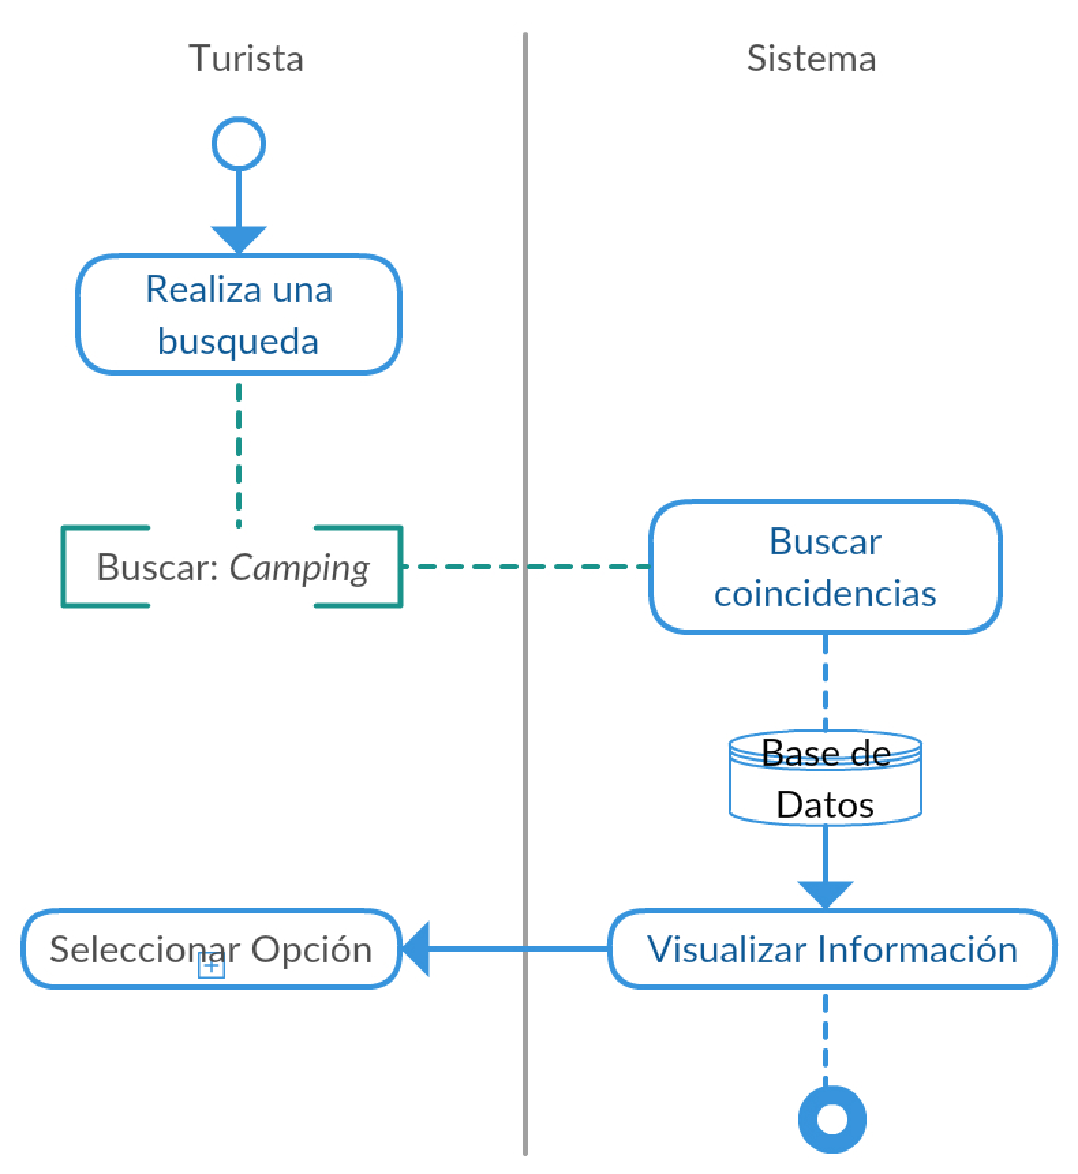
\includegraphics[scale=0.40]{/home/koskovi/Universidad/IngSoft/IS/Don-Oso/MN.pdf}
\caption{Diagrama de Modelo de Negocio asociado a la búsqueda}
\label{}\end{center}
\end{figure}


\end{document}